%\begin{figure}[H]
%    \centering
    \begin{tikzpicture}
        \pgfplotsset{
            width=1.0\textwidth,
            height=0.33\textheight
        }
        \begin{axis}
            [
                xbar=2pt,
                legend style={at={(0.5,-0.18)}, anchor=north,legend columns=-1},
                bar width = 5pt,
                xlabel= Execution Time (s),
                ylabel= Core,
                xmin=0,xmax=60,
                    ytick={0,1,2,3,4,5,6,7},
            ]
            \addplot coordinates { 
                (10,0)
                (10,1)
                (10.001,2)
                (10,3)
                (10,4)
                (10.001,5)
                (10,6)
                (10,7)
                };
            \addplot coordinates { 
                (16.3,0)
                (16.3,1)
                (16.3,2)
                (16.3,3)
                (16.3,4)
                (16.3,5)
                (16.3,6)
                (16.3,7)
                };
            \legend{NB, SN}
            \end{axis}
        \end{tikzpicture}
    % \caption{The Execution Time for DUT 1, where both benchmarks are compiled on oneAPI}
    \caption{Execution time}
%\end{figure}
